%--------------------
% Packages
% -------------------
\documentclass[11pt,a4paper]{article}
\usepackage[utf8x]{inputenc}
\usepackage[T1]{fontenc}
%\usepackage{gentium}
\usepackage{mathptmx} % Use Times Font
\usepackage[pdftex]{graphicx} % Required for including pictures
\usepackage{subfig}
\usepackage[pdftex,linkcolor=black,pdfborder={0 0 0}]{hyperref} % Format links for pdf
\usepackage{calc} % To reset the counter in the document after title page
\usepackage{enumitem} % Includes lists
\frenchspacing % No double spacing between sentences
\linespread{1.2} % Set linespace
\usepackage[a4paper, lmargin=0.1\paperwidth, rmargin=0.1\paperwidth, tmargin=0.05\paperheight, bmargin=0.05\paperheight]{geometry} %margins
%\usepackage{parskip}
\usepackage[all]{nowidow} % Tries to remove widows
\usepackage[protrusion=true,expansion=true]{microtype} % Improves typography, load after fontpackage is selected
\usepackage{lipsum} % Used for inserting dummy 'Lorem ipsum' text into the template
%-----------------------
% Set pdf information and add title, fill in the fields
%-----------------------
\hypersetup{ 	
pdfsubject = {},
pdftitle = {},
pdfauthor = {}
}
%-----------------------
% Begin document
%-----------------------
\begin{document} 

{\Large \textbf{CGGS-CW1 Report}}\\
\indent \indent {\large s2150204}

\subsubsection*{Section 1 Observations}

When the simuation is started on the mixed scene (video reference \texttt{<submission>/videos/mixed-scene.webm}) the objects fall and collide as expected. 
After a few seconds a notable event occurs, where we see that a larger rectangle collides with a smaller cube from the top, which causes the smaller cube to bounce out across the scene. 
This is due to the coefficient of restitution being 1, and represents an accurate simulation of a perfectly elastic collision. 
When the coefficient of restitution is reduced to 0.3 (that of wood), we see that the smaller ball doesn't bounce across the scene (video reference \texttt{<submission>/videos/mixed-scene-wood.webm}).

After a few more seconds we see another notable artifact in the mixed scene with a lowered coefficient of restitution. 
The oblong slides perpetually out of frame, when it should in fact stop moving. 
This behaviour is seen in all simulations with a lowered coefficient of restitution, such as in \texttt{stress-scene.txt} and \texttt{cube-scene.txt} (video references \texttt{<submission>/videos/stress-scene-wood.webm} and \texttt{<submission> /videos/cube-scene-wood.webm}. 
This could be explained by the lack of friction in the simulation, which could cause perpetual motion. 
Alternatively, floating point error in the integration code could mean that small errors are compounding to cause this problem. 

\subsubsection*{Section 2 Observations}

The constraint resolution program appears to work correctly.
When the simulation is started on the two chain scene (video reference \texttt{<submission>/videos/two-chain-scene.webm}), it works as expected, with each chain extending until they hit they ground, and then colliding with each other.
This is expected in this scene and the constraints appear to be working as expected. 
In the cube scene (video reference \texttt{<submission>/videos/ cube-scene.webm}), the cube made of constraints remains rigid and correctly spaced out as it collides with the ground, and all the cubes rotate correctly about the point that is constrained. 
There is some jittering as the cube maintains contact with the ground however.
In the two cylinder constrained scene (video reference \texttt{<submission>/videos/two-cylinder-scene.webm}), the cylinders bounce around but remain within the constrained distance, indicated a correctly functioning simulation.

There are few artifacts in the costrained scenes, except that sometimes constrained objects will clip into each other after the constraints are resolved. 
This is due to the constraints being resolved after collision in the code, which means that constraint resolution could result in interpenetration that is not resolved until the next frame. 
This makes it difficult to actually see as they are single frame artifacts. 
However, this could be the reason for jittering in the constrained cube scene, the cubes may be sliding into the ground after constraint resolution, causing jittering.

This constraint solver is also not incredibly performant, as it resolves constraints between all meshes in the scene, over and over again. 
This causes a lot of unnecessary calculations to be done, causing frame rate drops in a lot of cases. 
Moreover this method does not lead to fast constraint resolution, which means that the maximum number of iterations is often reached, causing further framedrops. 
However, as shown in the next section, this can be improved. 

\subsubsection*{Section 3 BPSS and Constraint Scheduling}
This section describes my implementation of the BPSS and constraint scheduling improvements.
These were implemented in \texttt{include/bpss.h} and \texttt{include/constraint\_scheduling.h} respectively. 
Figure \ref{fig:fps_scenes} shows how long frame generation takes for a variety of scenes before and after the improvements.
The extra stress scenes referred to can be found in \texttt{<submission>/data}. 

\subsubsection*{BPSS (Broad Phase Spatial Subdivision)}

My implementation of BPSS uses the commonly used Spatial Hashing method. 
This method divides the scene into a grid of cells, and then assigns each object to all the cells that it is in. 
Then, instead of resolving collisions over all the objects in the scene, we resolve collisions only between objects in the same cell.
This reduces unnecessary calculations, greatly improving the performance of the simulation. 

For the actual implementation, each cell was a \texttt{vector} which stored the meshes within the cell. 
The grid was implemented as a hashmap of cells, and is populated before resolving collisions. 
This populating step adds the mesh id to all cells within its bounding area, using a spatial hash function to map each cell location to a vector of mesh ids in the grid and then update the relevant vector.
Then, the program iterates over all the cells in the grid and resolves collisions between all the objects in each cell.
The end result was a single line call that significantly improved the performance factor of large simulations. 

Comparing performance with and without this optimizations demonstrates the success of BPSS for large scale simulations. 
Figure \ref{fig:fps_scenes} shows in the single object scene BPSS reduces performace, due to the overhead associated with it.
However with only 64 objects in the scene (stress\_64-scene) BPSS almost doubles performance, and with 9261 objects the base program does not run, while the BPSS enabled program remains above 20 FPS. 
This clearly demonstrates a successful optimization, able to handle 1000s of rigidbodies. 


\subsubsection*{Constraint Scheduling}

My implementation of the constraint scheduling method performs a depth-first search of constraints to resolve.
It resolves a constraint, by calling its constraint resolution function, and then recursively resolving constraints that are affected by the constraint. 
This is repeated until all constraints are resolved, or the depth cap is reached.

The actual implementation uses a map to store the related constraints and provide a search strategy for the depth first search.
At the beginning of constraint resolution, the map is populated with mesh index and constraint list pairs, in which each mesh index has a corresponding list of constraints it is part of. 
During constraint resolution, this map is referred to to get the list of all constraints that share a mesh id with the current constraint. 
This list is then recursively resolved in the same manner.
There is a depth cap to prevent unbounded recursion, and to prevent the program from hanging. 
Similar to the BPSS solution, it can be called in a single line to resolve all constraints in the scene.

As seen with BPSS, the performance increases given by this method improve with more constraints in the scene.
Figure \ref{fig:fps_scenes} shows similar performance in the two cylinder scene, which has only two constraints. 
In the two chain scene with sixteen constraints, we seen a larger performance increase, with performance boosts during the earlier stages of the simulation. 
Finally the cube scene, which has the most constraints, at 28, demonstrates the improvements fully, with the optimized simulation improving 7x over the baseline at some points. 
This clearly demonstrates an effective speedup. 


\subsection*{Submission Notes}

The submission includes the scripts used to collect data and graphs in the scripts folder, although the data collection may not work without the correct Section objects. 
All video files are in webm format as that was the only way to record screen captures on my computer. 



\begin{figure}[h]
    \centering 
    \begin{tabular}{cc} % 4x2 grid (2 columns)
        \subfloat[Two Cylinder scene with 2 constraints, demonstrating constraint scheduling overhead]{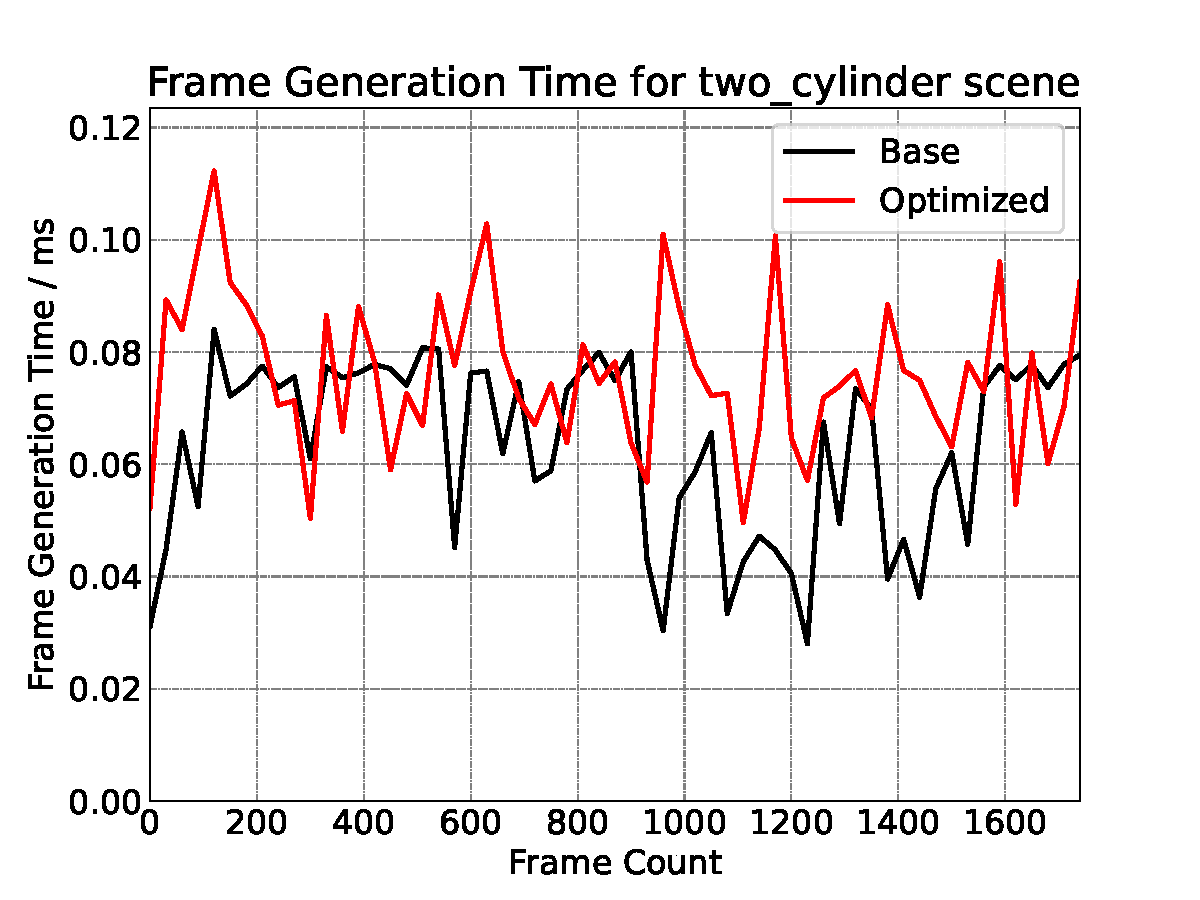
\includegraphics[height=0.2\paperheight]{figures/fps-two_cylinder-scene.pdf}} &
        \subfloat[Two Chain scene comparison with 16 constraints, demonstrating constraint scheduling improvements]{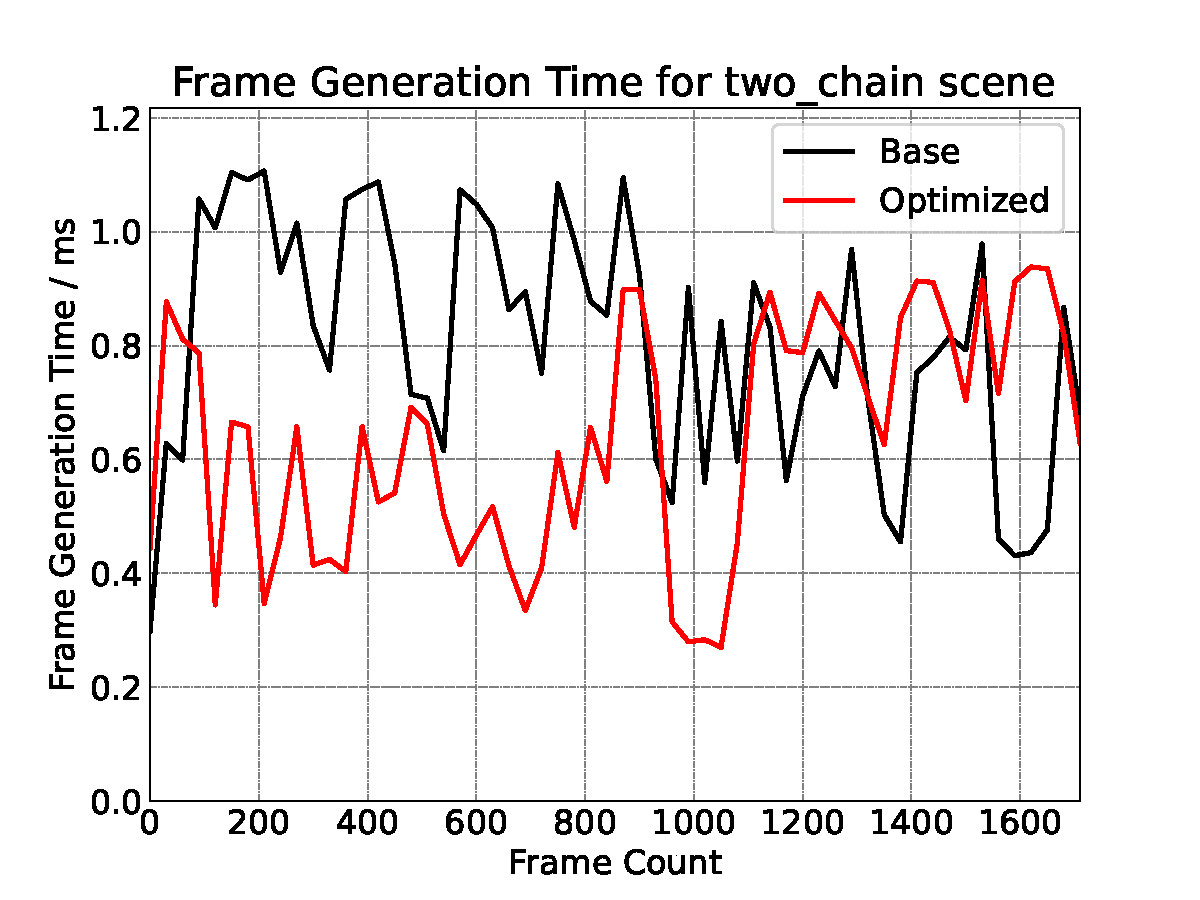
\includegraphics[height=0.2\paperheight]{figures/fps-two_chain-scene.pdf}} \\
        \subfloat[Cube scene comparison with 28 constraints, demonstrating constraint scheduling improvements]{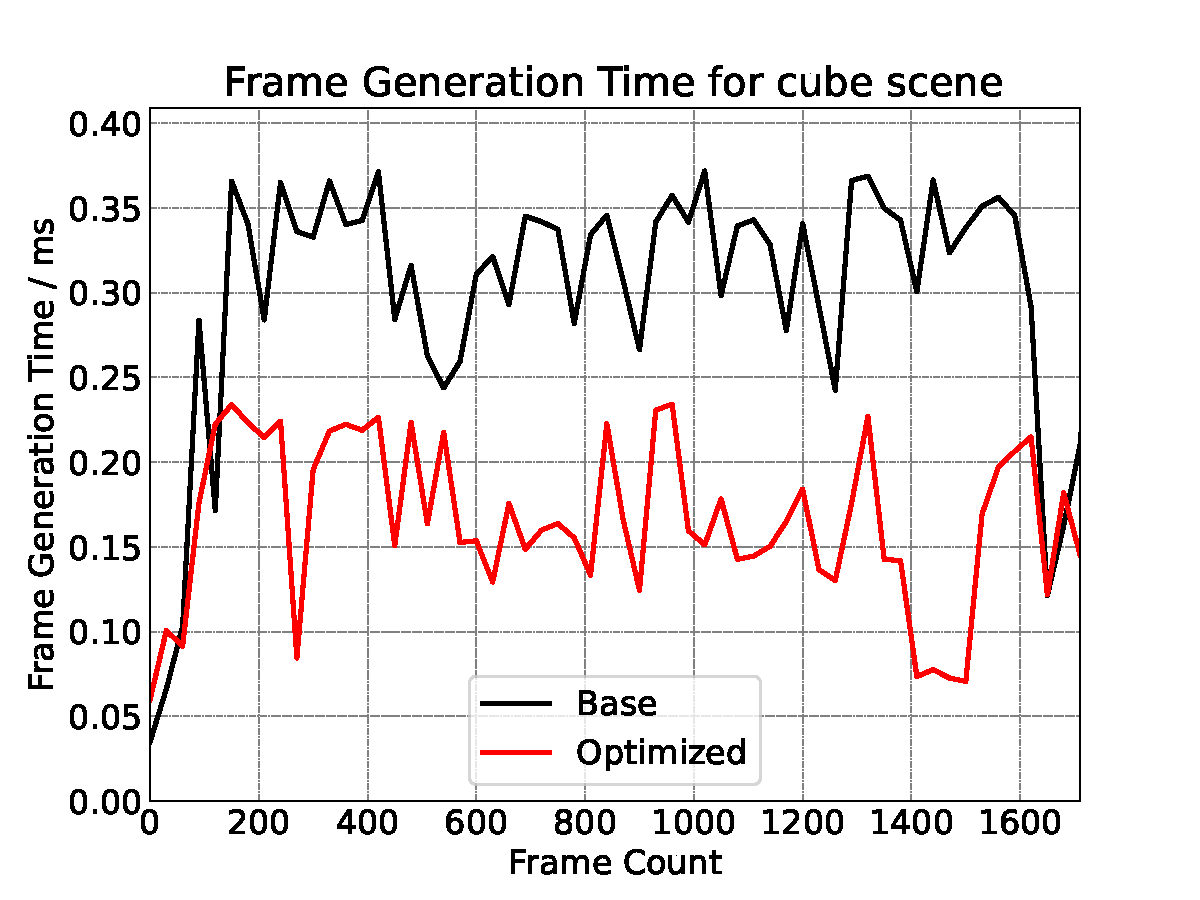
\includegraphics[height=0.2\paperheight]{figures/fps-cube-scene.pdf}} &
        \subfloat[Single Tet scene, demonstrating BPSS overhead]{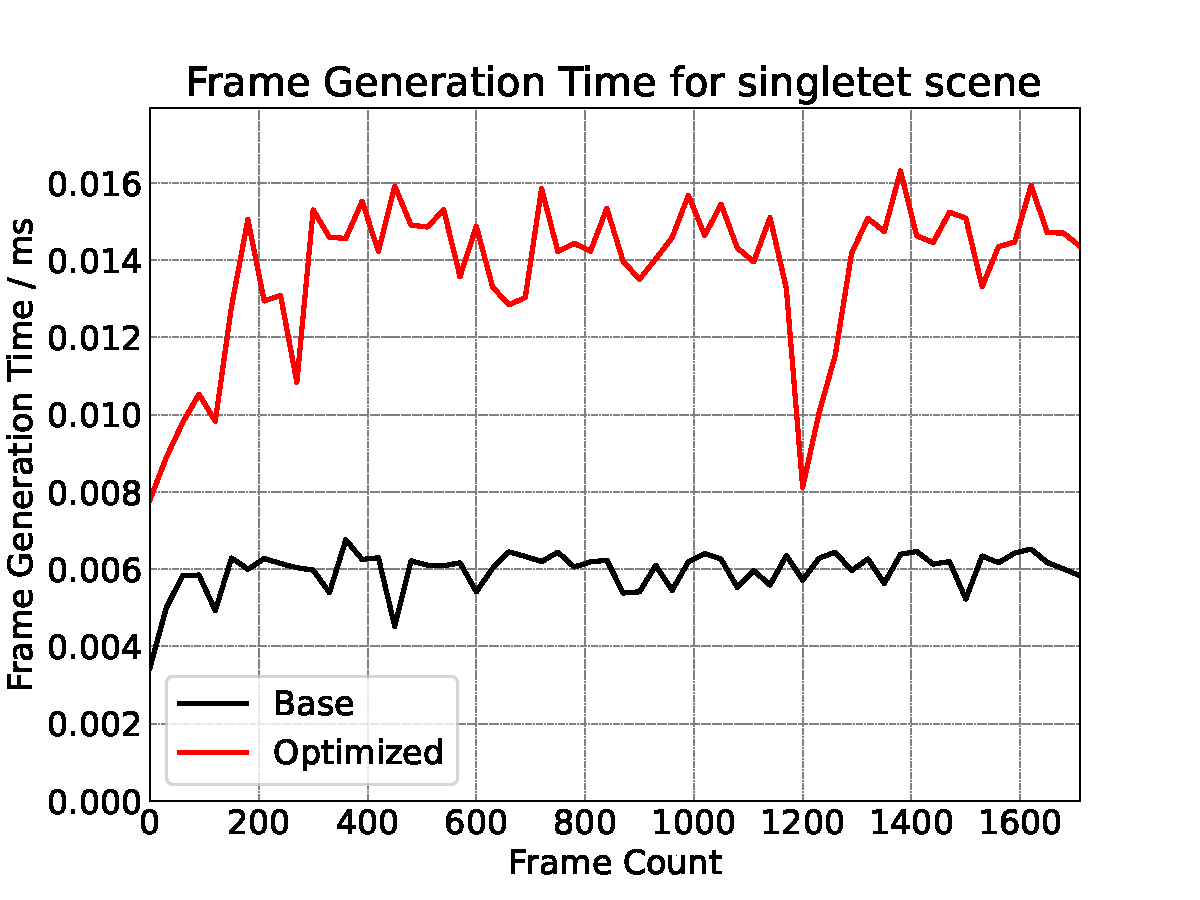
\includegraphics[height=0.2\paperheight]{figures/fps-singletet-scene.pdf}} \\
        \subfloat[Stress scene with 64 objects, showing doubled performance with BPSS]{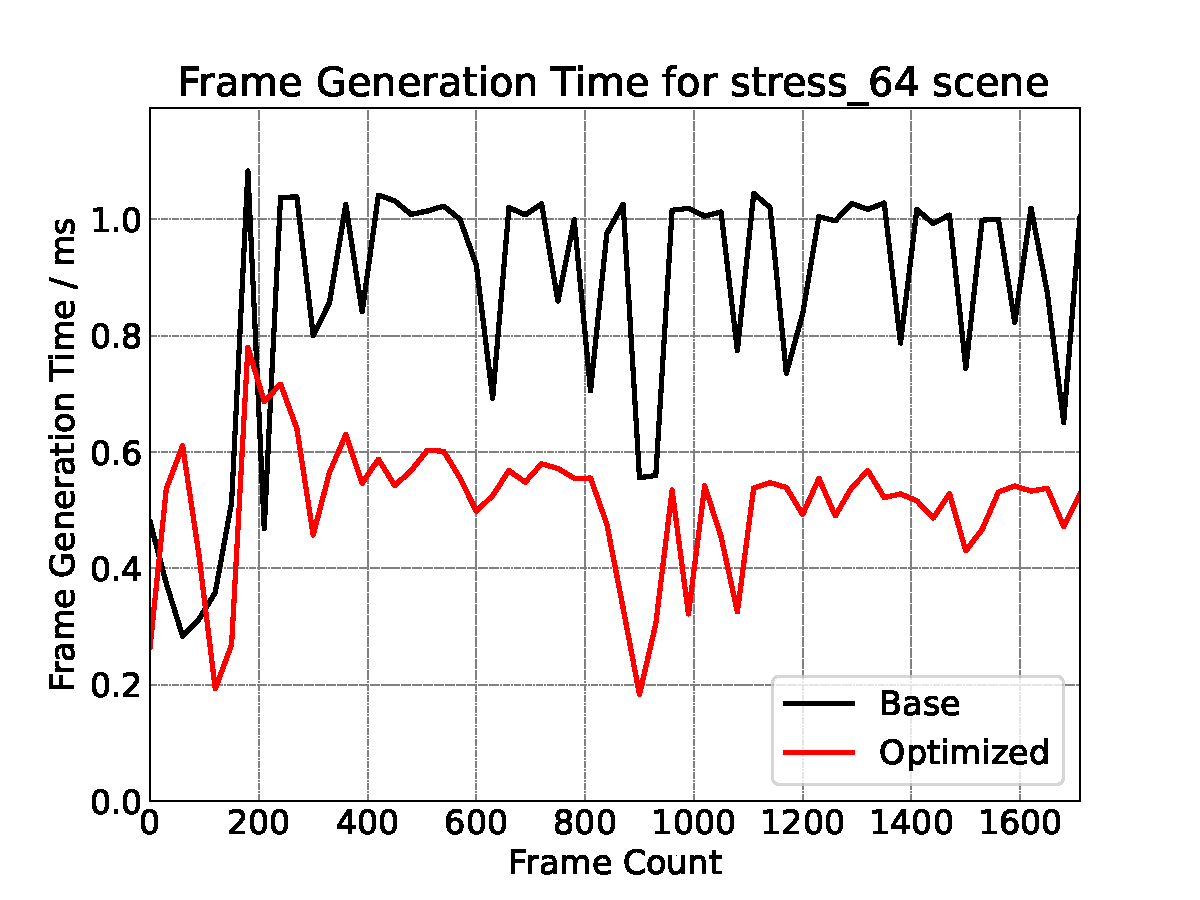
\includegraphics[height=0.2\paperheight]{figures/fps-stress_64-scene.pdf}} &
        \subfloat[Stress scene with 9261 objects, showing vastly superior performance over baseline]{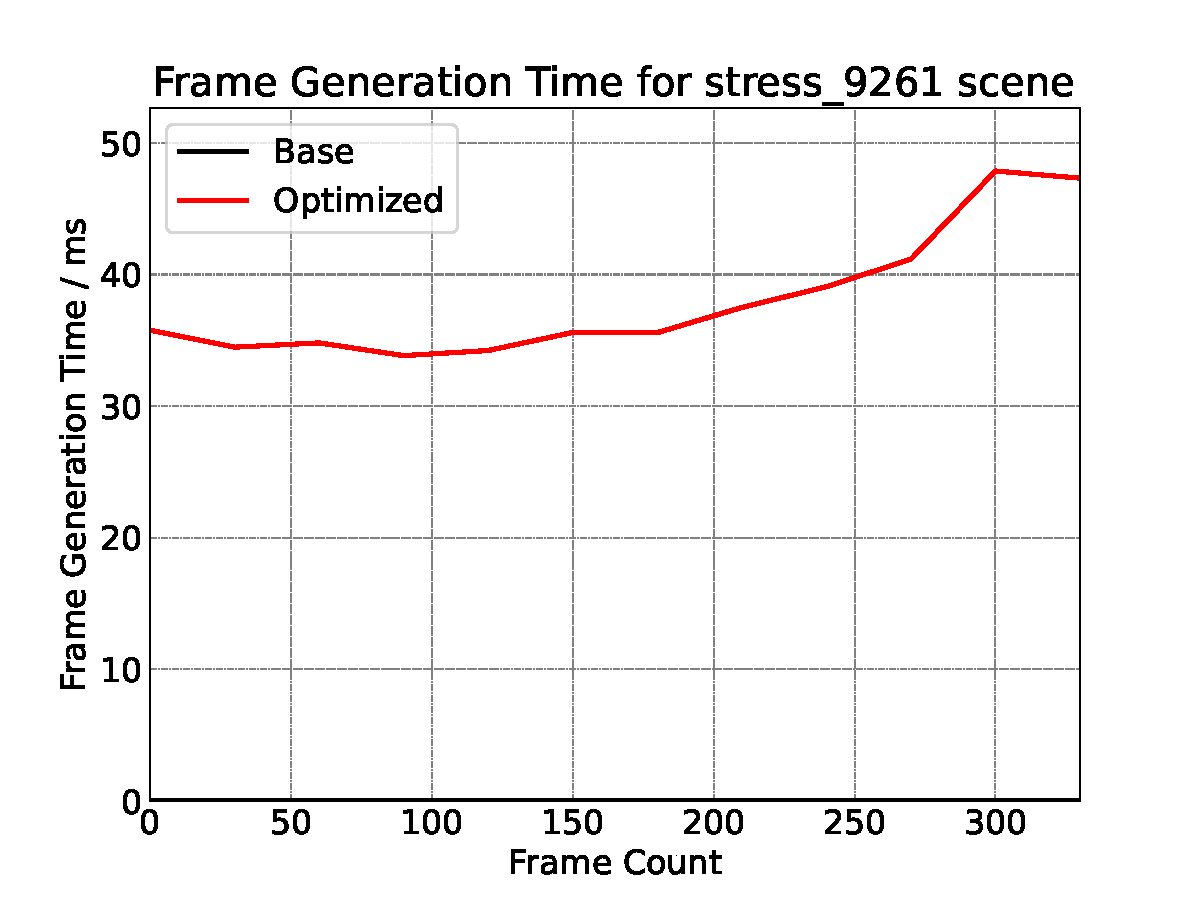
\includegraphics[height=0.2\paperheight]{figures/fps-stress_9261-scene.pdf}} \\
    \end{tabular}
    \caption{Frame generation time comparisons for all of the given scenes, showing before and after the BPSS and Constraint Scheduling improvements. The optimized line refers to the improved simulation with only the relevant optimization applied. All tests were on software built with \texttt{cmake -DCMAKE\_BUILD\_TYPE=Release ..}}
    \label{fig:fps_scenes}
\end{figure}
\end{document}
